\documentclass[a4paper]{article}

\usepackage[english]{babel}
\usepackage[utf8]{inputenc}
\usepackage{amsmath}
\usepackage{graphicx,caption,subcaption,float}
\usepackage[colorinlistoftodos]{todonotes}

\title{APC 524 / AST 506 / MAE 506 Software engineering for scientific computing
\\Assignment 4: Parallel programming with OpenMP and MPI}

\author{Hao Zhang, MAE, haozhang@princeton.edu}

\date{\today}

\begin{document}
\maketitle

\section{Comparison of serial, OpenMP, and MPI}
\subsection{Single thread, Serial, OpenMP, MPI}
      \begin{figure}[H]
        \centering
        \begin{subfigure}[b]{0.32\textwidth}   
            \centering 
            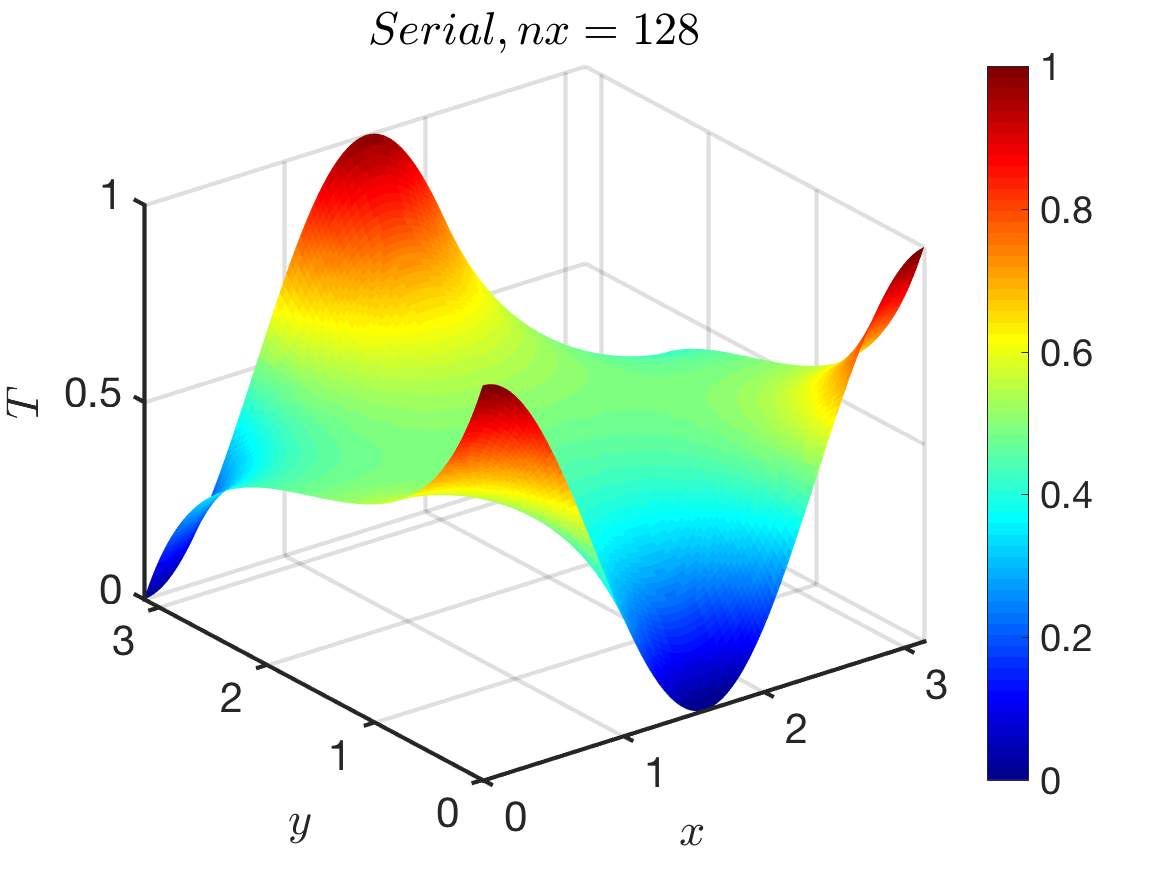
\includegraphics[width=\textwidth]{./Figure/heat_serial_nx128.png} 
        \end{subfigure}
        \
        \begin{subfigure}[b]{0.32\textwidth}   
            \centering 
            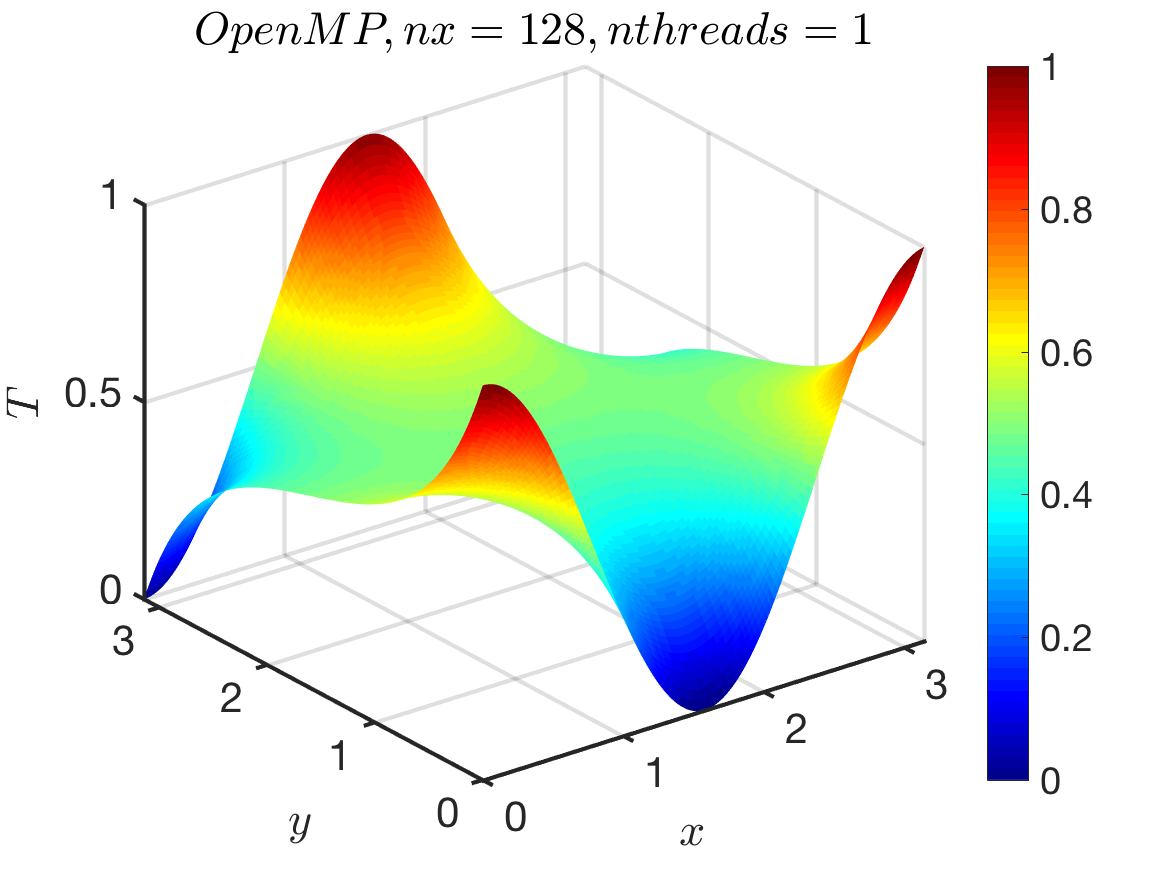
\includegraphics[width=\textwidth]{./Figure/heat_omp_nx128_nth1.png}  
        \end{subfigure}
        \
                \begin{subfigure}[b]{0.32\textwidth}   
            \centering 
            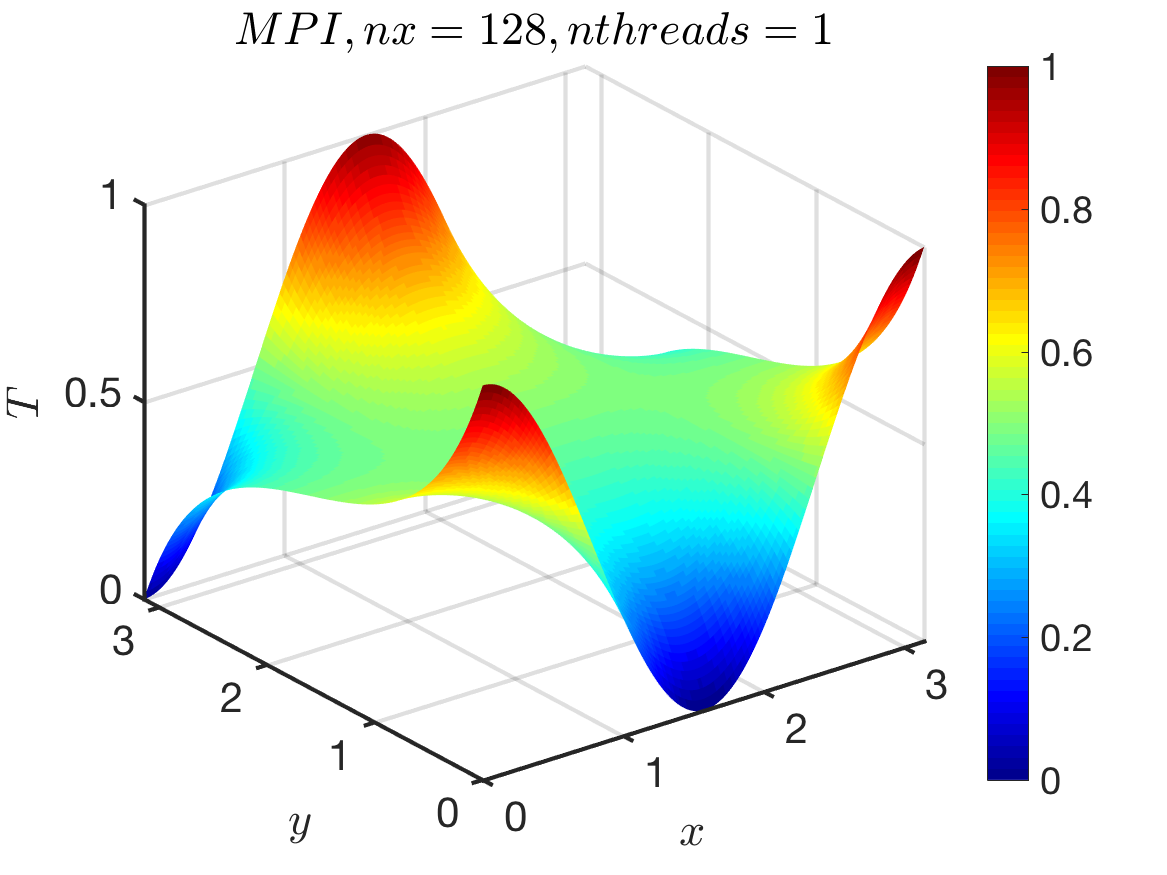
\includegraphics[width=\textwidth]{./Figure/heat_mpi_nx128_nth1_rank0.png} 
        \end{subfigure}
        \caption{Temperature field computed by serial, OpenMP, and MPI with a single thread, grid size $128\times128$}
    \end{figure}
    
    \subsection{Multiple thread, OpenMP}
    
    \subsection{Multiple thread, MPI}
    
\end{document}